\documentclass[letterpaper,12pt]{article}
\usepackage{array}
\usepackage{threeparttable}
\usepackage{geometry}
\usepackage{amsmath}
\geometry{letterpaper,tmargin=1in,bmargin=1in,lmargin=1.25in,rmargin=1.25in}
\usepackage{fancyhdr,lastpage}
\pagestyle{fancy}
\lhead{}
\chead{}
\rhead{}
\lfoot{}
\cfoot{}
\rfoot{\footnotesize\textsl{Page \thepage\ of \pageref{LastPage}}}
\renewcommand\headrulewidth{0pt}
\renewcommand\footrulewidth{0pt}
\usepackage[format=hang,font=normalsize,labelfont=bf]{caption}
\usepackage{listings}
\lstset{frame=single,
  language=Python,
  showstringspaces=false,
  columns=flexible,
  basicstyle={\small\ttfamily},
  numbers=none,
  breaklines=true,
  breakatwhitespace=true
  tabsize=3
}
\usepackage{amsmath}
\usepackage{amssymb}
\usepackage{amsthm}
\usepackage{harvard}
\usepackage{setspace}
\usepackage{float,color}
\usepackage[pdftex]{graphicx}
\usepackage{hyperref}
\hypersetup{colorlinks,linkcolor=red,urlcolor=blue}
\theoremstyle{definition}
\newtheorem{theorem}{Theorem}
\newtheorem{acknowledgement}[theorem]{Acknowledgement}
\newtheorem{algorithm}[theorem]{Algorithm}
\newtheorem{axiom}[theorem]{Axiom}
\newtheorem{case}[theorem]{Case}
\newtheorem{claim}[theorem]{Claim}
\newtheorem{conclusion}[theorem]{Conclusion}
\newtheorem{condition}[theorem]{Condition}
\newtheorem{conjecture}[theorem]{Conjecture}
\newtheorem{corollary}[theorem]{Corollary}
\newtheorem{criterion}[theorem]{Criterion}
\newtheorem{definition}[theorem]{Definition}
\newtheorem{derivation}{Derivation} % Number derivations on their own
\newtheorem{example}[theorem]{Example}
\newtheorem{exercise}[theorem]{Exercise}
\newtheorem{lemma}[theorem]{Lemma}
\newtheorem{notation}[theorem]{Notation}
\newtheorem{problem}[theorem]{Problem}
\newtheorem{proposition}{Proposition} % Number propositions on their own
\newtheorem{remark}[theorem]{Remark}
\newtheorem{solution}[theorem]{Solution}
\newtheorem{summary}[theorem]{Summary}
%\numberwithin{equation}{section}
\bibliographystyle{aer}
\newcommand\ve{\varepsilon}
\newcommand\boldline{\arrayrulewidth{1pt}\hline}


\begin{document}

\begin{flushleft}
  \textbf{\large{Problem Set \#4}} \\
  MACS 30100, Dr. Evans \\
  Soo Wan Kim
\end{flushleft}

\noindent\textbf{Problem 1} \\
\textbf {Part (a)}

\begin{figure}[h!]
  
\includegraphics[width=\linewidth]{1a.png}
  \caption{1a}
\end{figure}

\noindent
\textbf {Part (b)} 

\noindent
Test PDF values: \\
$$ \left[
\begin{array}{c c}
0.0019079 		& 		 0.00123533 \\
0.00217547 		& 		0.0019646 \\
\end{array} \right] 
$$

\noindent\textbf {Part (c).} 

\begin{figure}[h!]
  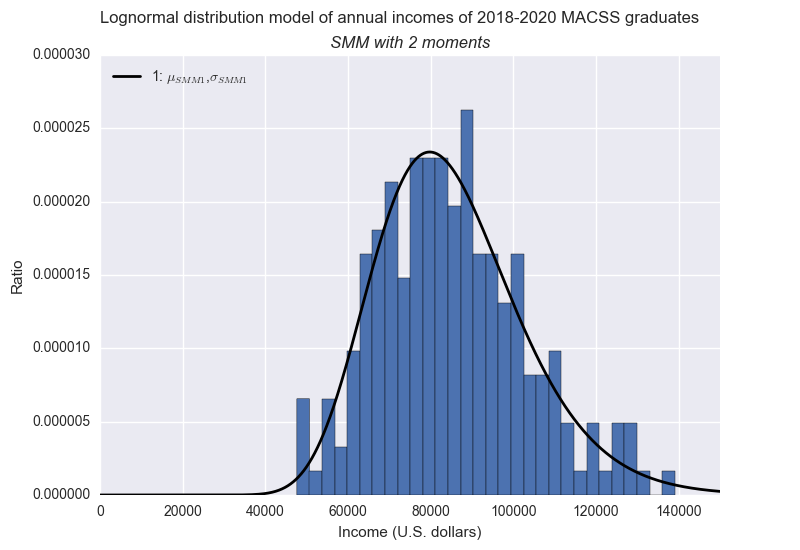
\includegraphics[width=\linewidth]{1c.png}
  \caption{1c}
\end{figure}

\noindent
With estimated parameter values $\mu$ = 11.330637236 and $\sigma$ = 0.209229370701, the value of the SMM criterion function is 5.55966141266e-15.\\\\
Data moments and model moments compared:\\
Average, standard deviation of income data = (85276.8236063, 17992.542128)\\
Mean, standard deviation of model (one-step estimation) = (85276.8280721, 17992.543083)\\\\
\noindent
The data and model moments are very nearly the same.\\

\noindent\textbf {Part (d).} \\

\begin{figure}[h!]
  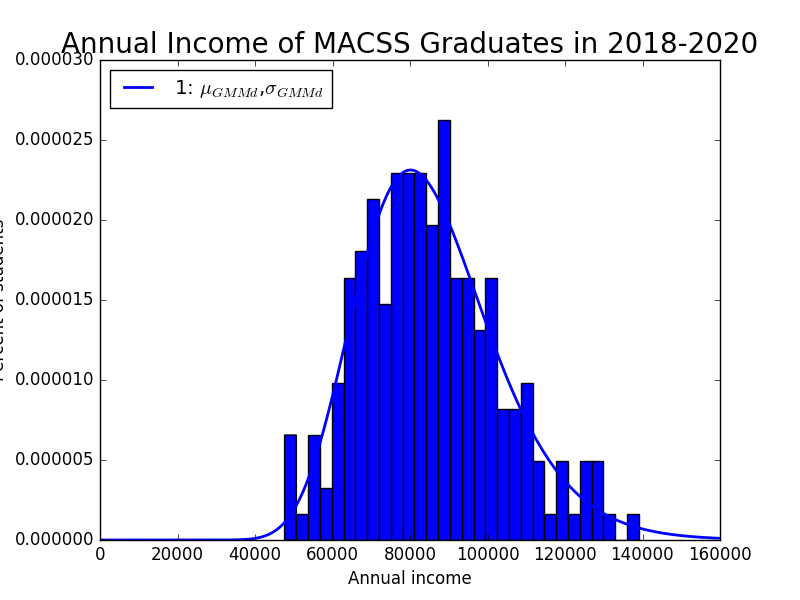
\includegraphics[width=\linewidth]{1d.png}
  \caption{1d}
\end{figure}

\noindent
With the estimated parameter values $\mu$ = 11.3306372141 and $\sigma$ = 0.209229359136, the value of the SMM criterion function is 0.000176839034035.\\\\
Data moments and model moments compared:\\
Average, standard deviation of income data = (85276.8236063, 17992.542128)\\
Mean, standard deviation of model (one-step estimation) = (85276.8280721, 17992.543083)\\
Mean, standard deviation of model (two-step estimation) = (85276.8259939, 17992.5416292)\\\\
\noindent
Although the one-step estimation provides a good fit for the two moments chosen, the two-step estimation produces model moments even closer to the data moments.

\end{document}
